%package list
\documentclass{article}
\usepackage[top=3cm, bottom=3cm, outer=3cm, inner=3cm]{geometry}
\usepackage{multicol}
\usepackage{graphicx}
\usepackage{url}
\usepackage{hyperref}
\usepackage{array}
\newcolumntype{x}[1]{>{\centering\arraybackslash\hspace{0pt}}p{#1}}
\usepackage{natbib}
\usepackage{pdfpages}
\usepackage{multirow}
\usepackage[normalem]{ulem}
\useunder{\uline}{\ul}{}
\usepackage{svg}
\usepackage{xcolor}
\usepackage{listings}
\lstdefinestyle{ascii-tree}{
    literate={├}{|}1 {─}{--}1 {└}{+}1 
  }
\lstset{basicstyle=\ttfamily,
  showstringspaces=false,
  commentstyle=\color{red},
  keywordstyle=\color{blue}
}
%\usepackage{booktabs}
\usepackage{caption}
\usepackage{subcaption}
\usepackage{float}
\usepackage{array}

% Comment
\usepackage{verbatim}

\newcolumntype{M}[1]{>{\centering\arraybackslash}m{#1}}
\newcolumntype{N}{@{}m{0pt}@{}}


%%%%%%%%%%%%%%%%%%%%%%%%%%%%%%%%%%%%%%%%%%%%%%%%%%%%%%%%%%%%%%%%%%%%%%%%%%%%
%%%%%%%%%%%%%%%%%%%%%%%%%%%%%%%%%%%%%%%%%%%%%%%%%%%%%%%%%%%%%%%%%%%%%%%%%%%%
\newcommand{\itemEmail}{rzapata@unsa.edu.pe}
\newcommand{\itemStudent}{Reyser Julio Zapata Butron}
\newcommand{\itemCourse}{Análisis Y Diseño de Algoritmos}
\newcommand{\itemCourseCode}{1702231}
\newcommand{\itemSemester}{IV}
\newcommand{\itemUniversity}{Universidad Nacional de San Agustín de Arequipa}
\newcommand{\itemFaculty}{Facultad de Ingeniería de Producción y Servicios}
\newcommand{\itemDepartment}{Departamento Académico de Ingeniería de Sistemas e Informática}
\newcommand{\itemSchool}{Escuela Profesional de Ingeniería de Sistemas}
\newcommand{\itemAcademic}{2024 - B}
\newcommand{\itemInput}{03 diciembre 2024}
\newcommand{\itemOutput}{03 diciembre 2024}
\newcommand{\itemPracticeNumber}{08}
\newcommand{\itemTheme}{Búsqueda en profundidad}
\newcommand{\itemPracticeDuration}{02 horas}
%%%%%%%%%%%%%%%%%%%%%%%%%%%%%%%%%%%%%%%%%%%%%%%%%%%%%%%%%%%%%%%%%%%%%%%%%%%%
%%%%%%%%%%%%%%%%%%%%%%%%%%%%%%%%%%%%%%%%%%%%%%%%%%%%%%%%%%%%%%%%%%%%%%%%%%%%

\usepackage[english,spanish]{babel}
\usepackage[utf8]{inputenc}
\AtBeginDocument{\selectlanguage{spanish}}
\renewcommand{\figurename}{Figura}
\renewcommand{\refname}{Referencias}
\renewcommand{\tablename}{Tabla} %esto no funciona cuando se usa babel
\AtBeginDocument{%
	\renewcommand\tablename{Tabla}
}

\usepackage{fancyhdr}
\pagestyle{fancy}
\fancyhf{}
\setlength{\headheight}{30pt}
\renewcommand{\headrulewidth}{1pt}
\renewcommand{\footrulewidth}{1pt}
\fancyhead[L]{\raisebox{-0.2\height}{
\includegraphics[width=3cm]{img/logo_episunsa.png}}}
\fancyhead[C]{\fontsize{7}{7}\selectfont	\itemUniversity \\ \itemFaculty \\ \itemDepartment \\ \itemSchool \\ \textbf{\itemCourse}}
\fancyhead[R]{\raisebox{-0.2\height}{
\includegraphics[width=1.2cm]{img/logo_abet}}}
\fancyfoot[L]{Reyser Julio Zapata Butrón}
\fancyfoot[C]{\itemCourse}
\fancyfoot[R]{Página \thepage}

% Estilos del Código
\usepackage{listings}
\usepackage{color, colortbl}
\definecolor{dkgreen}{rgb}{0,0.6,0}
\definecolor{gray}{rgb}{0.5,0.5,0.5}
\definecolor{codebackground}{rgb}{89, 0.97, 0.90}
\definecolor{tablebackground}{rgb}{0.8, 0, 0}

\lstset{
  language=C++,                  
  basicstyle=\ttfamily\footnotesize,
  keywordstyle=\color{blue},     
  commentstyle=\color{dkgreen},    
  stringstyle=\color{red},       
  backgroundcolor= \color{codebackground},
  numbers=left,                  
  numberstyle=\tiny\color{gray},
  stepnumber=1,                  
  numbersep=5pt,                
  showspaces=false,              
  showstringspaces=false,      
  showtabs=false,                
  frame=single,                  
  captionpos=b,                  %
}

\begin{document}
	\vspace*{10px}
	
	\begin{center}	
		\fontsize{17}{17} \textbf{ Informe de Laboratorio \itemPracticeNumber}
	\end{center}

 %% TABLA %%
 
	\centerline{\textbf{\Large Tema: \itemTheme}}

	\begin{flushright}
		\begin{tabular}{|M{2.5cm}|N|}
			\hline 
			\rowcolor{tablebackground}
			\color{white} \textbf{Nota}  \\
			\hline 
			     \\[30pt]
			\hline 			
		\end{tabular}
	\end{flushright}	

	\begin{table}[H]
		\begin{tabular}{|x{4.7cm}|x{4.8cm}|x{4.8cm}|}
			\hline 
			\rowcolor{tablebackground}
			\color{white} \textbf{Estudiante} & \color{white}\textbf{Escuela}  & \color{white}\textbf{Asignatura}   \\
			\hline 
			{\itemStudent \par \itemEmail} & \itemSchool & {\itemCourse \par Semestre: \itemSemester \par Código: \itemCourseCode}     \\
			\hline 			
		\end{tabular}
	\end{table}		
	
	\begin{table}[H]
		\begin{tabular}{|x{4.7cm}|x{4.8cm}|x{4.8cm}|}
			\hline 
			\rowcolor{tablebackground}
			\color{white}\textbf{Laboratorio} & \color{white}\textbf{Tema}  & \color{white}\textbf{Duración}   \\
			\hline 
			\itemPracticeNumber & \itemTheme & \itemPracticeDuration   \\
			\hline 
		\end{tabular}
	\end{table}
	
	\begin{table}[H]
		\begin{tabular}{|x{4.7cm}|x{4.8cm}|x{4.8cm}|}
			\hline 
			\rowcolor{tablebackground}
			\color{white}\textbf{Semestre académico} & \color{white}\textbf{Fecha de inicio}  & \color{white}\textbf{Fecha de entrega}   \\
			\hline 
			\itemAcademic & \itemInput &  \itemOutput  \\
			\hline 
		\end{tabular}
	\end{table}

 %% CONTENIDO %%
\section{Código base}
    El siguiente código presentado, es la base para la realización de los ejerción propuestos\\
    \lstinputlisting[language=C++, caption={base.cpp}, numbers=left]{src/base.cpp}

\section{Ejercicios Propuestos}
    \subsection{Casos extremos. ¿Cuál es el resultado de GRAPHdfs(G) cuando G.adj es 0? ¿Y cuando G.V es 1?
    }

       \subsubsection*{Cuando \texttt{G.adj} es 0}
            Si la matriz de adyacencia \texttt{G.adj} está completamente llena de ceros, esto indica que el grafo no tiene ninguna arista; es decir, todos los vértices son aislados. En este escenario, la función \texttt{GRAPHdfs(G)} realizará lo siguiente:
            
            \begin{itemize}
                \item \textbf{Inicialización:} El contador \texttt{cnt} se establece en 0 y todos los elementos del arreglo \texttt{pre[]} se inicializan a -1, indicando que ningún vértice ha sido visitado.
                
                \item \textbf{Recorrido de Vértices:} La función iterará sobre cada vértice del grafo. Dado que no hay aristas, la condición \texttt{G.adj[v][w] == 1} nunca se cumplirá, por lo que no se realizarán llamadas recursivas a \texttt{dfsR()}.
                
                \item \textbf{Asignación de Números de Orden:} Cada vértice se considerará una componente conectada por sí mismo. Por lo tanto, \texttt{dfsR()} se llamará para cada vértice individualmente, asignando un número de orden secuencial a cada uno.
                
                \item \textbf{Resultado Final:} El vector \texttt{order} contendrá todos los vértices en orden ascendente desde 0 hasta \texttt{G.V - 1}, y el arreglo \texttt{pre[v]} reflejará el orden en que fueron visitados, que coincidirá con su índice debido a la ausencia de aristas.
            \end{itemize}
    
        \subsubsection*{Cuando \texttt{G.V} es 1}
            Si el grafo tiene únicamente un vértice (\texttt{G.V = 1}), la función \texttt{GRAPHdfs(G)} operará de la siguiente manera:
            
            \begin{itemize}
                \item \textbf{Inicialización:} Similar al caso anterior, \texttt{cnt} se establece en 0 y \texttt{pre[0]} se inicializa a -1.
                
                \item \textbf{Recorrido de Vértices:} Solo hay un vértice que considerar. La condición \texttt{pre[v] == -1} se cumple para \texttt{v = 0}, por lo que se llamará a \texttt{dfsR(G, 0, 0, order)}.
                
                \item \textbf{Ejecución de \texttt{dfsR()}:} 
                \begin{itemize}
                    \item Se asigna \texttt{pre[0] = 0} y \texttt{order} se actualiza para incluir el vértice 0.
                    \item Se intenta iterar sobre posibles adyacencias, pero dado que \texttt{G.adj[0][w]} es 0 para cualquier \texttt{w}, no se realizarán más llamadas recursivas.
                    \item La función termina después de asignar el número de orden al único vértice.
                \end{itemize}
                
                \item \textbf{Resultado Final:} El vector \texttt{order} contendrá solo el vértice 0, y \texttt{pre[0]} será 0, reflejando que el único vértice ha sido visitado primero.
            \end{itemize}
        
    \subsection{Base de la recursión. ¿Cuál es la base de la recursión en la función dfsR()?}
        La base de la recursión en la función \texttt{dfsR()} se alcanza cuando se intenta explorar un vértice que ya ha sido visitado o cuando no hay más vértices adyacentes no visitados para explorar desde el vértice actual. Específicamente:
    
        \begin{itemize}
            \item \textbf{Vértice ya visitado:} Si durante la exploración de los adyacentes de un vértice \texttt{v}, se encuentra un vértice \texttt{w} tal que \texttt{pre[w] != -1}, esto indica que \texttt{w} ya ha sido visitado. En este caso, no se realiza una llamada recursiva y se continúa con el siguiente vértice adyacente.
            
            \item \textbf{Sin vértices adyacentes no visitados:} Si un vértice \texttt{v} no tiene vértices adyacentes \texttt{w} tales que \texttt{G.adj[v][w] == 1} y \texttt{pre[w] == -1}, la función \texttt{dfsR()} termina su ejecución para \texttt{v}, retornando al vértice desde el cual se realizó la llamada recursiva.
        \end{itemize}

    \subsection{Realiza una búsqueda en profundidad en el grafo dado por las siguientes listas de adyacencia. Haga un rastreo de la búsqueda.
            \[
            \begin{array}{r|l}
            0  & 1, 4 \\
            1  & 2, 5 \\
            2  & 3 \\
            3  & 7 \\
            4  & 8 \\
            5  & 4 \\
            6  & 5, 10, 2 \\
            7  & 11, 6 \\
            8  & 9 \\
            9  & 5, 8 \\
            10 & 9 \\
            11 & 10 \\
            \end{array}
            \]
    }    

    \textbf{Ejecución del código}
            \begin{figure}[H]
            	\centering
             	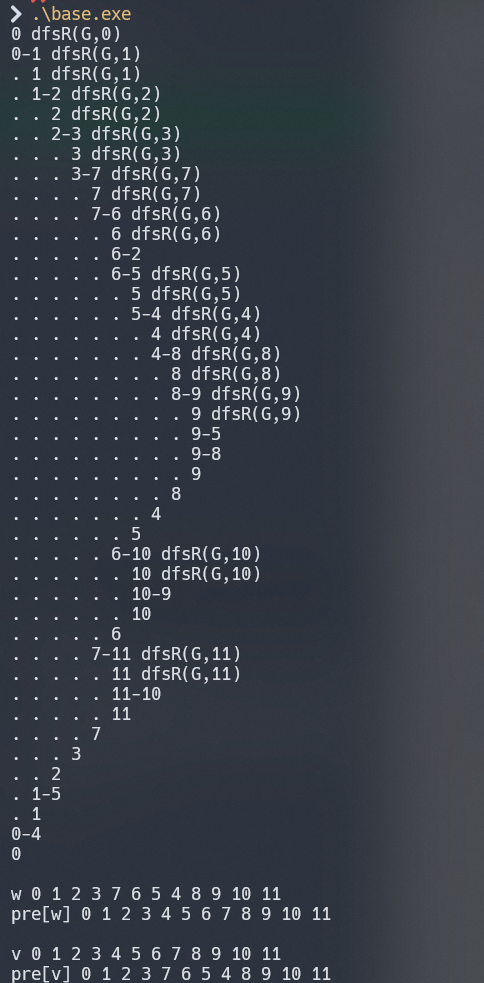
\includegraphics[width=0.7\textwidth,keepaspectratio]{img/exercise3.png}
            \end{figure}
 
%%% REPOSITORIO DE GITHUB %%%
\section{Repositorio de Github}
	\begin{itemize}
		\item Repositorio de Github donde se encuentra el actual laboratorio \\
		\url{https://github.com/ReyserLynnn/ada-lab-b-24b/tree/main/laboratorio08/src}

        \item Repositorio de Github donde se encuentran los laboratorios del curso\\
		\url{https://github.com/ReyserLynnn/ada-lab-b-24b.git}
	\end{itemize}

\begin{comment}
\section{Referencias}
\begin{itemize}			
	\item \url{https://dialnet.unirioja.es/servlet/articulo?codigo=4573315}
\end{itemize}	    
\end{comment}

\end{document}